\documentclass[12pt,a4paper]{article}
\usepackage[utf8]{inputenc}
\usepackage[spanish]{babel}
\usepackage{graphicx}
\usepackage{geometry}
\usepackage{hyperref}
\usepackage{listings}
\usepackage{xcolor}
\usepackage{titlesec}
\usepackage{booktabs}
\usepackage{caption}

\geometry{margin=2.5cm}

% Configuracion de colores para codigo
\definecolor{codegreen}{rgb}{0,0.6,0}
\definecolor{codegray}{rgb}{0.5,0.5,0.5}
\definecolor{codepurple}{rgb}{0.58,0,0.82}
\definecolor{backcolour}{rgb}{0.95,0.95,0.92}

\lstdefinestyle{mystyle}{
    backgroundcolor=\color{backcolour},   
    commentstyle=\color{codegreen},
    keywordstyle=\color{magenta},
    numberstyle=\tiny\color{codegray},
    stringstyle=\color{codepurple},
    basicstyle=\ttfamily\footnotesize,
    breaklines=true,                 
    captionpos=b,                    
    numbers=left,                    
    numbersep=5pt,                  
    tabsize=2,
    literate={á}{{\'a}}1 {é}{{\'e}}1 {í}{{\'i}}1 {ó}{{\'o}}1 {ú}{{\'u}}1 {ñ}{{\~n}}1
}
\lstset{style=mystyle}

\captionsetup[figure]{name=Figura}

\begin{document}

% --- CARÁTULA ---
\begin{titlepage}
    \centering
    \vspace*{1.5cm}
    {\huge\bfseries Laboratorio 6 - Parte 3: \par}
    {\huge\bfseries BluePrints API - React - UI \par}
    \vspace{1cm}
    {\Large mediante Autenticación JWT y Redux Toolkit \par}
    \vspace{3cm}
    {\large María Paula Rodríguez Muñoz \par}
    {\large Juan Andrés Suárez \par}
    {\large Juan Pablo Nieto \par}
    {\large Tomás Felipe Ramírez \par}
    \vfill
    \vfill
    {\large Materia: ARSW \par}
    {\large \today \par}
\end{titlepage}

\newpage

\section{Introducción}
Este laboratorio extiende un proyecto previo para la gestión de blueprints mediante la creación de un cliente moderno en **React + Vite**. Su objetivo es implementar una interfaz de usuario reactiva que gestione y visualice planos geométricos, consumiendo una REST API protegida con autenticación JWT y criptografía RSA. La aplicación sigue una arquitectura por capas en el frontend e integra procesamiento visual en tiempo real mediante un lienzo (Canvas). Este reporte detalla la implementación técnica, los objetivos alcanzados y las evidencias de funcionamiento del sistema final.

\section{Objetivos}

\subsection{Objetivo General}
Desarrollar un cliente moderno en React para la gestión de blueprints que implemente autenticación segura con JWT, manejo de estado global con Redux Toolkit y una arquitectura desacoplada por capas para la integración con APIs REST, garantizando la mantenibilidad y escalabilidad del sistema.

\subsection{Objetivos Específicos}
\begin{itemize}
    \item Implementar una interfaz de usuario mediante componentes de React que facilite la visualización interactiva de planos en el navegador.
    \item Integrar Redux Toolkit para la gestión centralizada de la información de autores, planos y el plano seleccionado actualmente.
    \item Desarrollar una capa de servicios (Service Layer) con un patrón de fachada que permita conmutar entre almacenamiento Mock y producción sin alterar la lógica de los componentes.
    \item Configurar autenticacion de usuarios mediante tokens JWT almacenados de forma persistente en \texttt{localStorage} para asegurar el acceso a recursos protegidos.
    \item Implementar rutas protegidas mediante componentes de orden superior y manejo de estados asincronos para una experiencia de usuario fluida.
    \item Validar el funcionamiento del cliente mediante una suite de pruebas unitarias y de integración con Vitest.
\end{itemize}

\subsection{Diagrama de Componentes}
El sistema se organiza pedagógicamente en los siguientes módulos:
\begin{itemize}
    \item \textbf{UI Components:} Pages (Blueprints, Login) y componentes especializados como \texttt{BlueprintCanvas}.
    \item \textbf{State Manager:} Redux Store con un slice dedicado a la lógica de negocio de los blueprints.
    \item \textbf{Service Layer:} Capa de abstracción encargada de la comunicación con el origen de datos (Mock/API).
\end{itemize}

\newpage

\section{Ejecución del Proyecto}

\subsection{Requisitos Previos}
\begin{itemize}
    \item Node.js 18+ instalado en el sistema operativo.
    \item Gestor de paquetes npm/npx configurado.
    \item Docker Desktop activo para el despliegue de contenedores.
\end{itemize}

\subsection{Configuración de Entorno}
La aplicación utiliza variables de entorno inyectadas mediante un archivo \texttt{.env} para configurar la URL base de la API:
\begin{lstlisting}
VITE_API_BASE_URL=http://localhost:8080/api
VITE_USE_MOCK=true
\end{lstlisting}

\subsection{Compilación y Ejecución}
Para iniciar el proyecto en modo de desarrollo, se deben ejecutar los siguientes comandos desde la terminal:
\begin{lstlisting}[language=bash]
# Instalacion de dependencias del proyecto
npm install
# Levantar el servidor de desarrollo Vite
npm run dev
\end{lstlisting}

La aplicación estará accesible en el navegador a través de la dirección \texttt{http://localhost:5173}.

\subsection{Endpoints Principales}
Todas las operaciones sobre la ruta \texttt{/api/**} requieren un token JWT válido adjunto en las cabeceras de autorización.

\subsubsection{Servicio de Autenticación}
\begin{lstlisting}[basicstyle=\ttfamily\scriptsize]
POST /auth/login
Content-Type: application/json
{
  "username": "student",
  "password": "student123"
}
\end{lstlisting}

\subsubsection{Consulta de Blueprints de un Autor}
\begin{lstlisting}[basicstyle=\ttfamily\scriptsize]
GET /api/v1/blueprints/{author}
Authorization: Bearer <access_token>
\end{lstlisting}

\newpage

\subsubsection{Creación de un Nuevo Blueprint}
\begin{lstlisting}[basicstyle=\ttfamily\scriptsize]
POST /api/v1/blueprints
{
  "author": "john",
  "name": "workshop",
  "points": [{"x": 10, "y": 10}, {"x": 50, "y": 50}]
}
# Codigo de respuesta esperado: 201 Created
\end{lstlisting}

\subsection{Ejecución de Suite de Pruebas}
Se validan los componentes y la lógica de estado mediante pruebas automatizadas:
\begin{lstlisting}[language=bash]
# Ejecucion de pruebas unitarias
npm test
\end{lstlisting}

\begin{figure}[h]
    \centering
    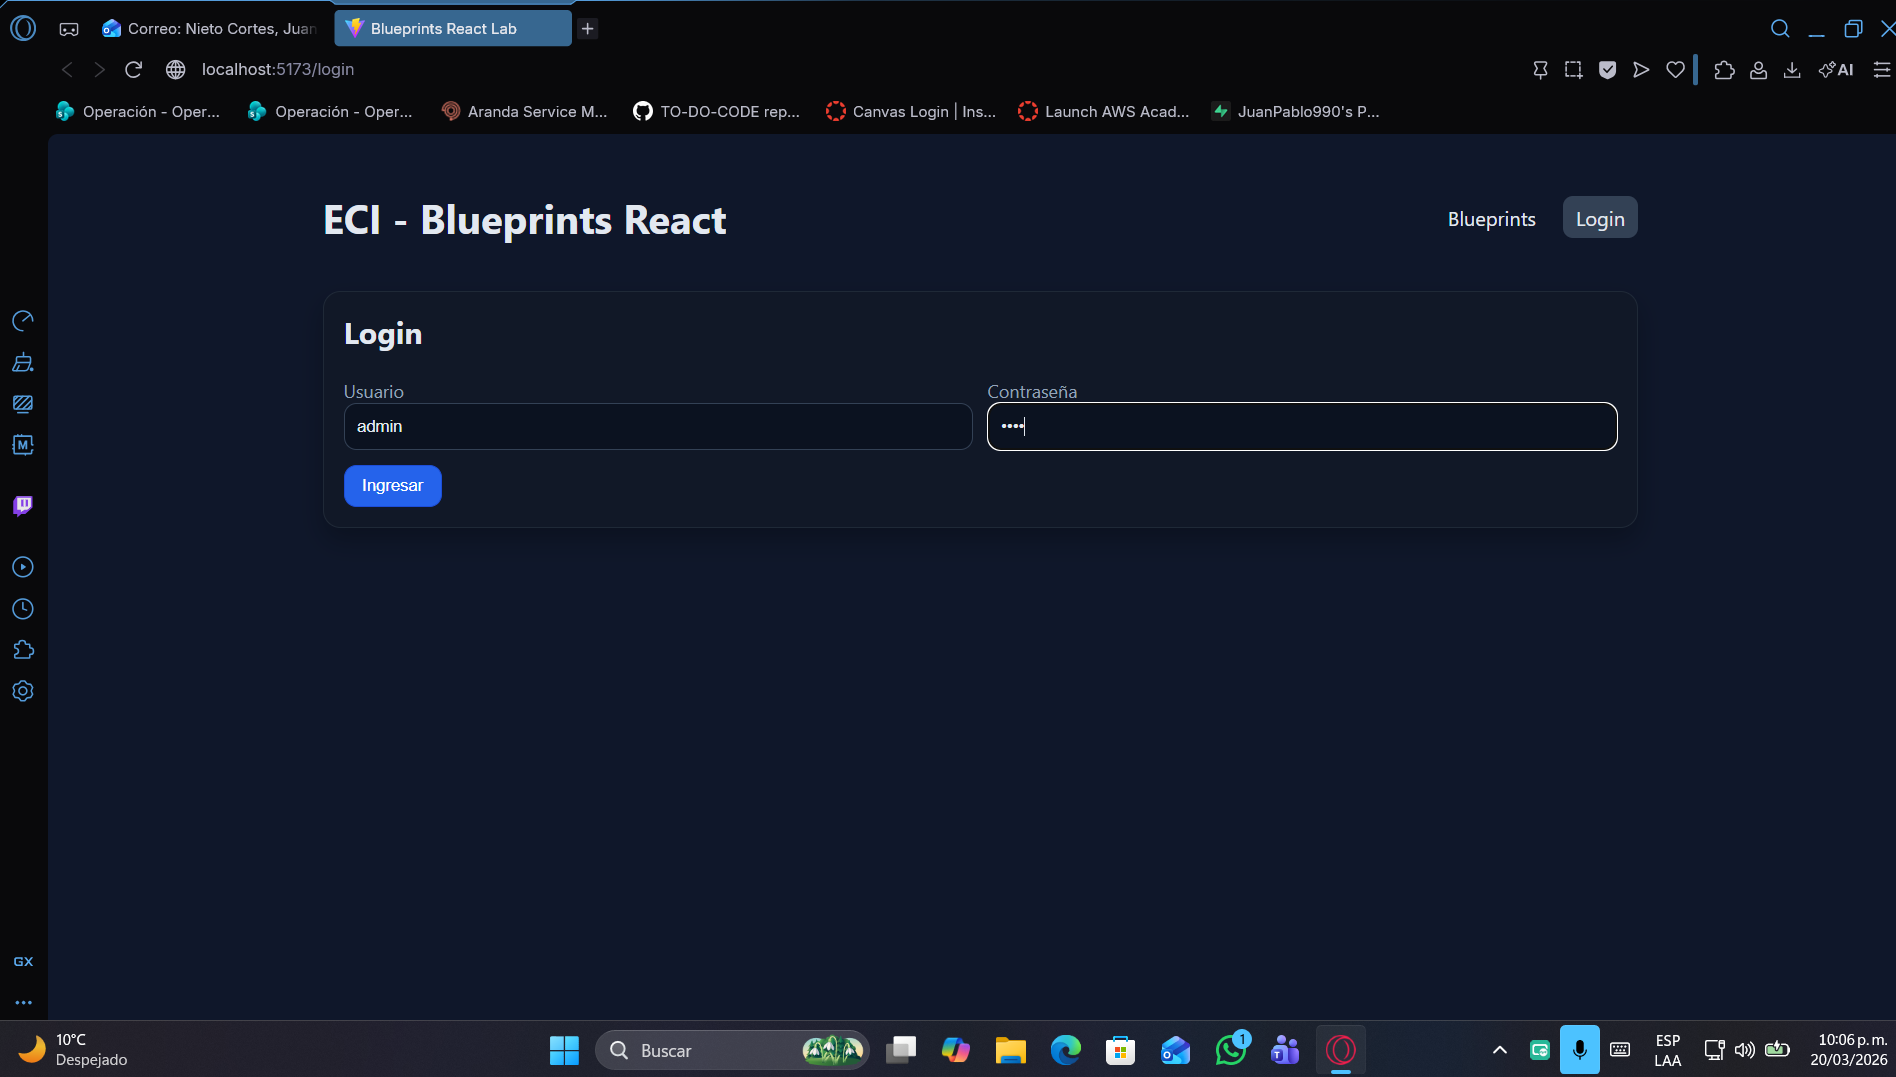
\includegraphics[width=0.8\textwidth]{login.png}
    \caption{Figura 1: Resumen de ejecución de pruebas unitarias con Vitest}
\end{figure}

\newpage

\section{Evidencias de Ejecución}

\subsection{Proceso de autenticación JWT}
Para acceder a los recursos protegidos se debe ingresar al sistema mediante la pantalla de login, la cual retorna un token JWT firmado.
\begin{figure}[h]
    \centering
    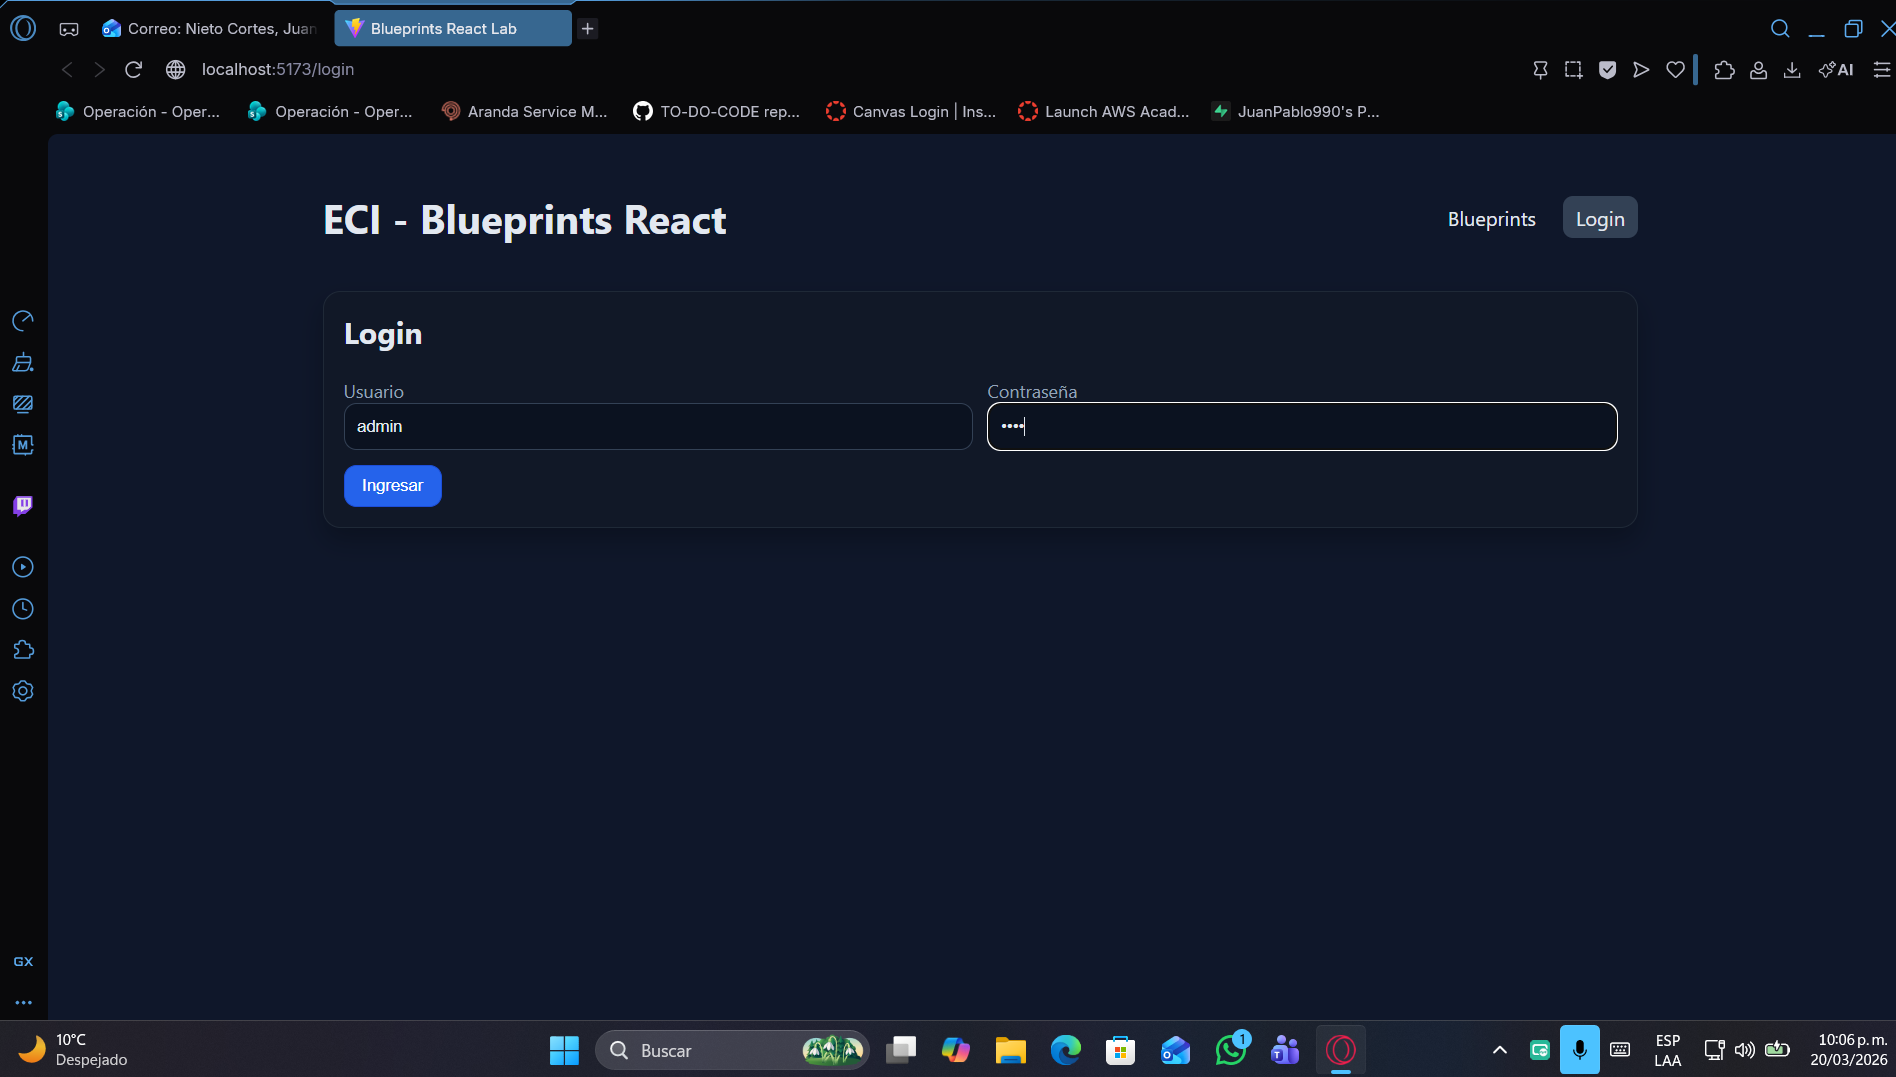
\includegraphics[width=0.9\textwidth]{login.png}
    \caption{Figura 2: Solicitud de autenticación al endpoint /auth/login}
\end{figure}

\begin{figure}[h]
    \centering
    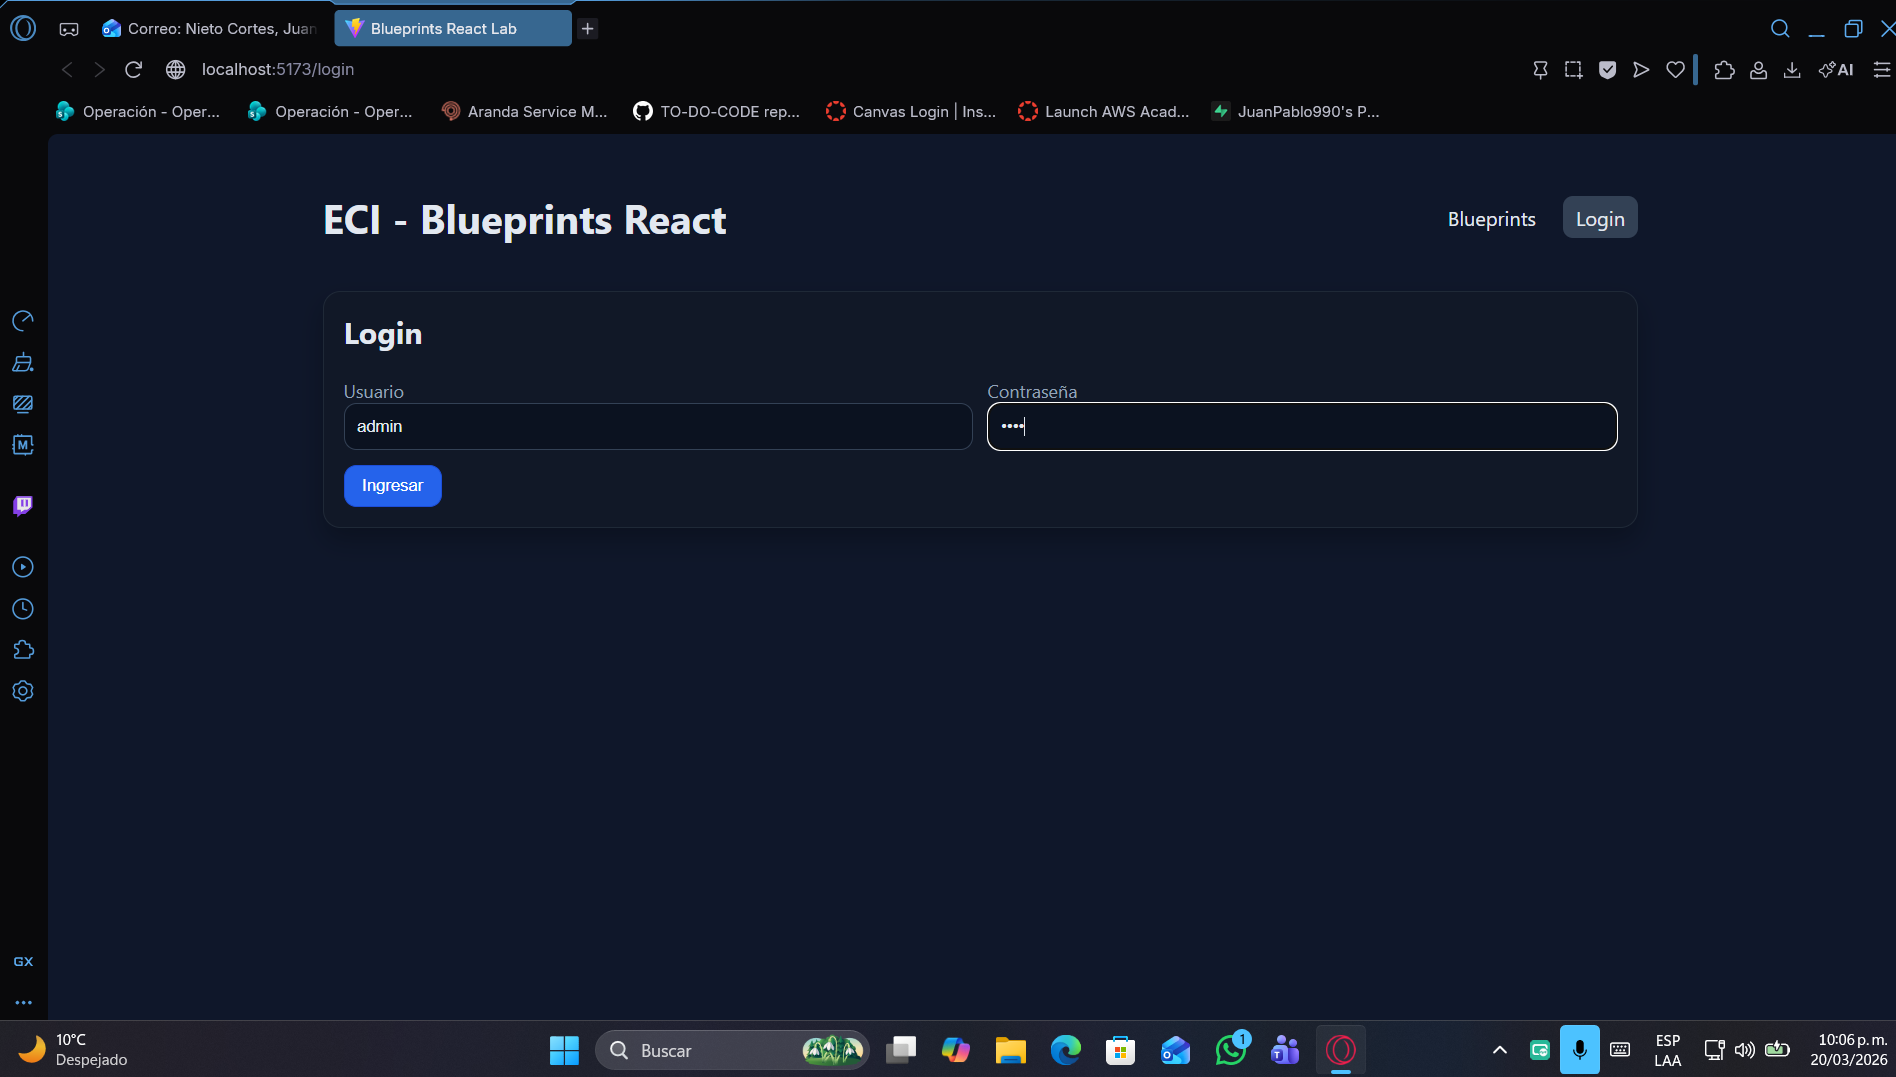
\includegraphics[width=0.9\textwidth]{login.png}
    \caption{Figura 3: Token JWT capturado exitosamente por el frontend}
\end{figure}

\newpage

\subsection{Consulta por Autor y Cálculo de Puntos}
Se verificó la funcionalidad de búsqueda por autor, la cual muestra la tabla de planos y calcula dinámicamente el total de puntos geométricos.
\begin{figure}[h]
    \centering
    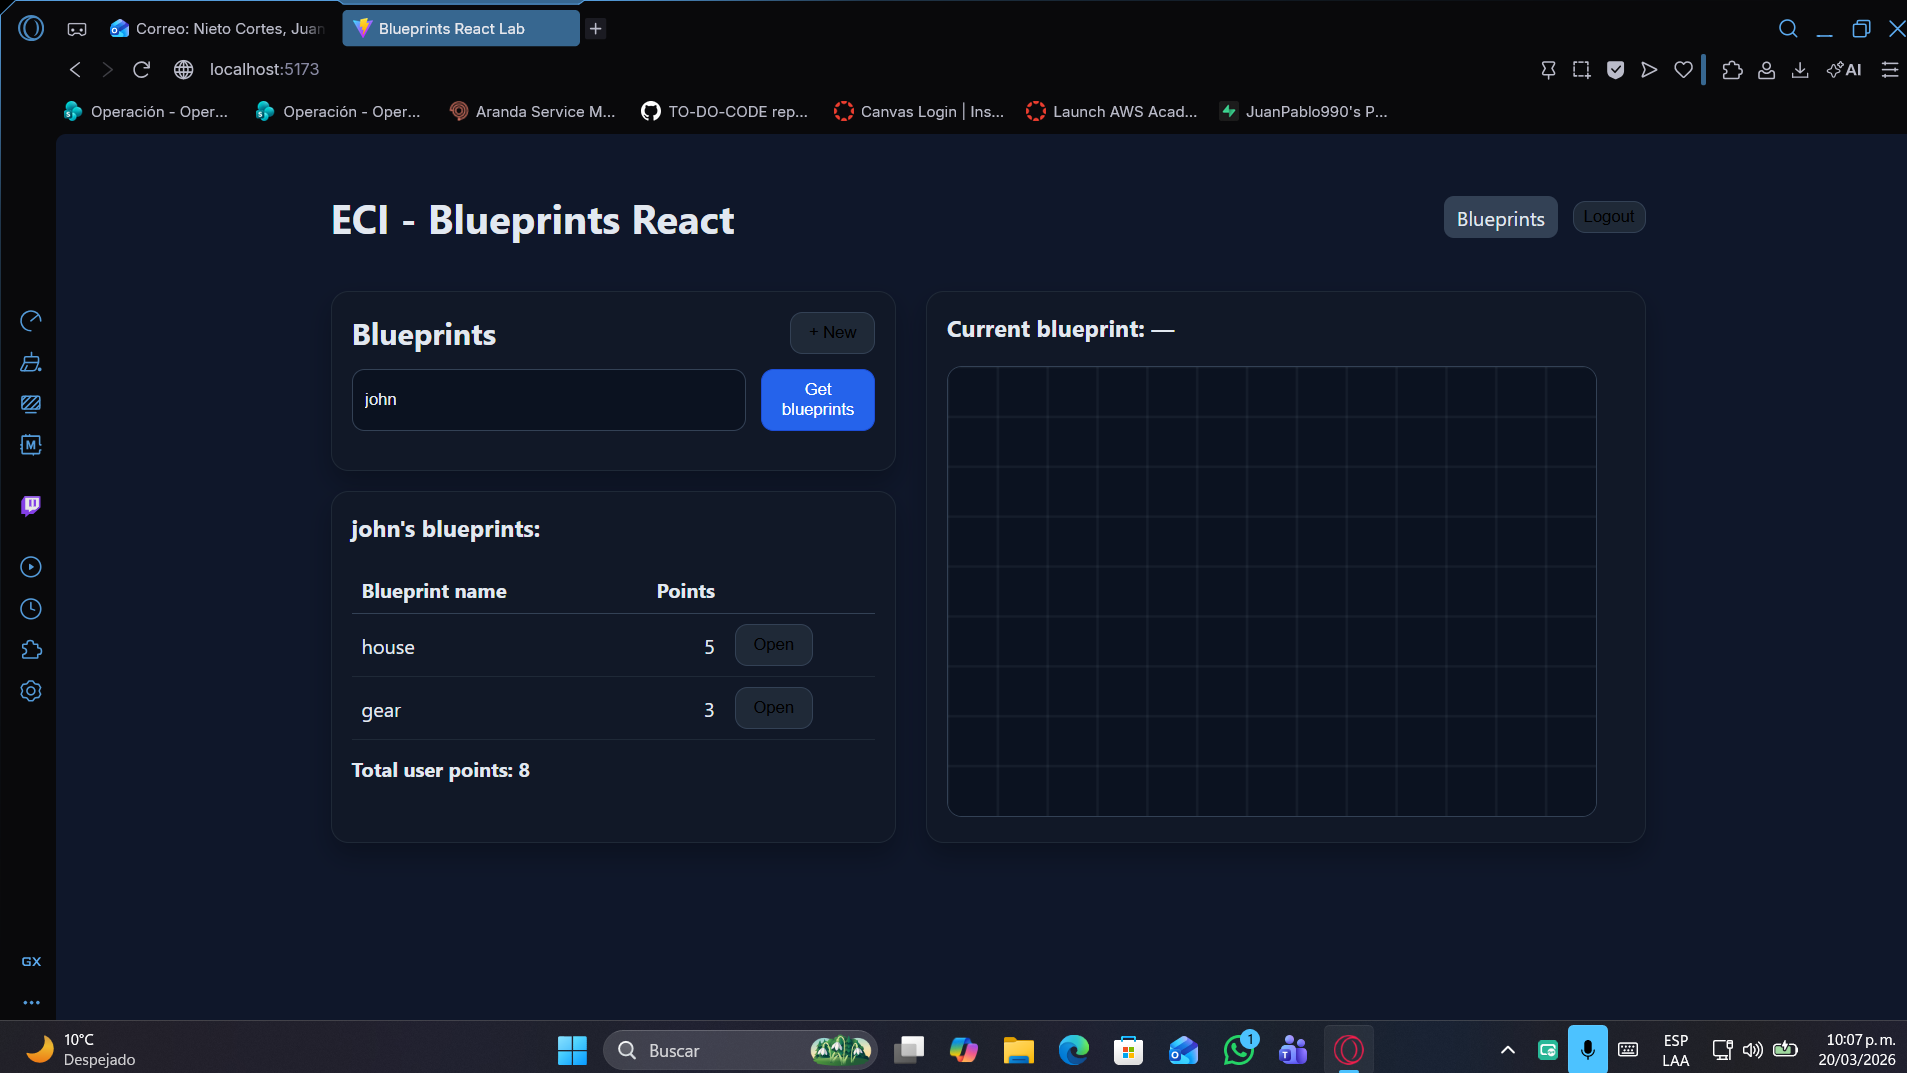
\includegraphics[width=0.95\textwidth]{busqueda de john.png}
    \caption{Figura 4: Interfaz de búsqueda y visualización de planos del autor john}
\end{figure}

\newpage

\subsection{Visualización en Canvas Interactiva}
Al abrir un plano, se grafican los puntos y segmentos correspondientes en el lienzo centralizado.
\begin{figure}[h]
    \centering
    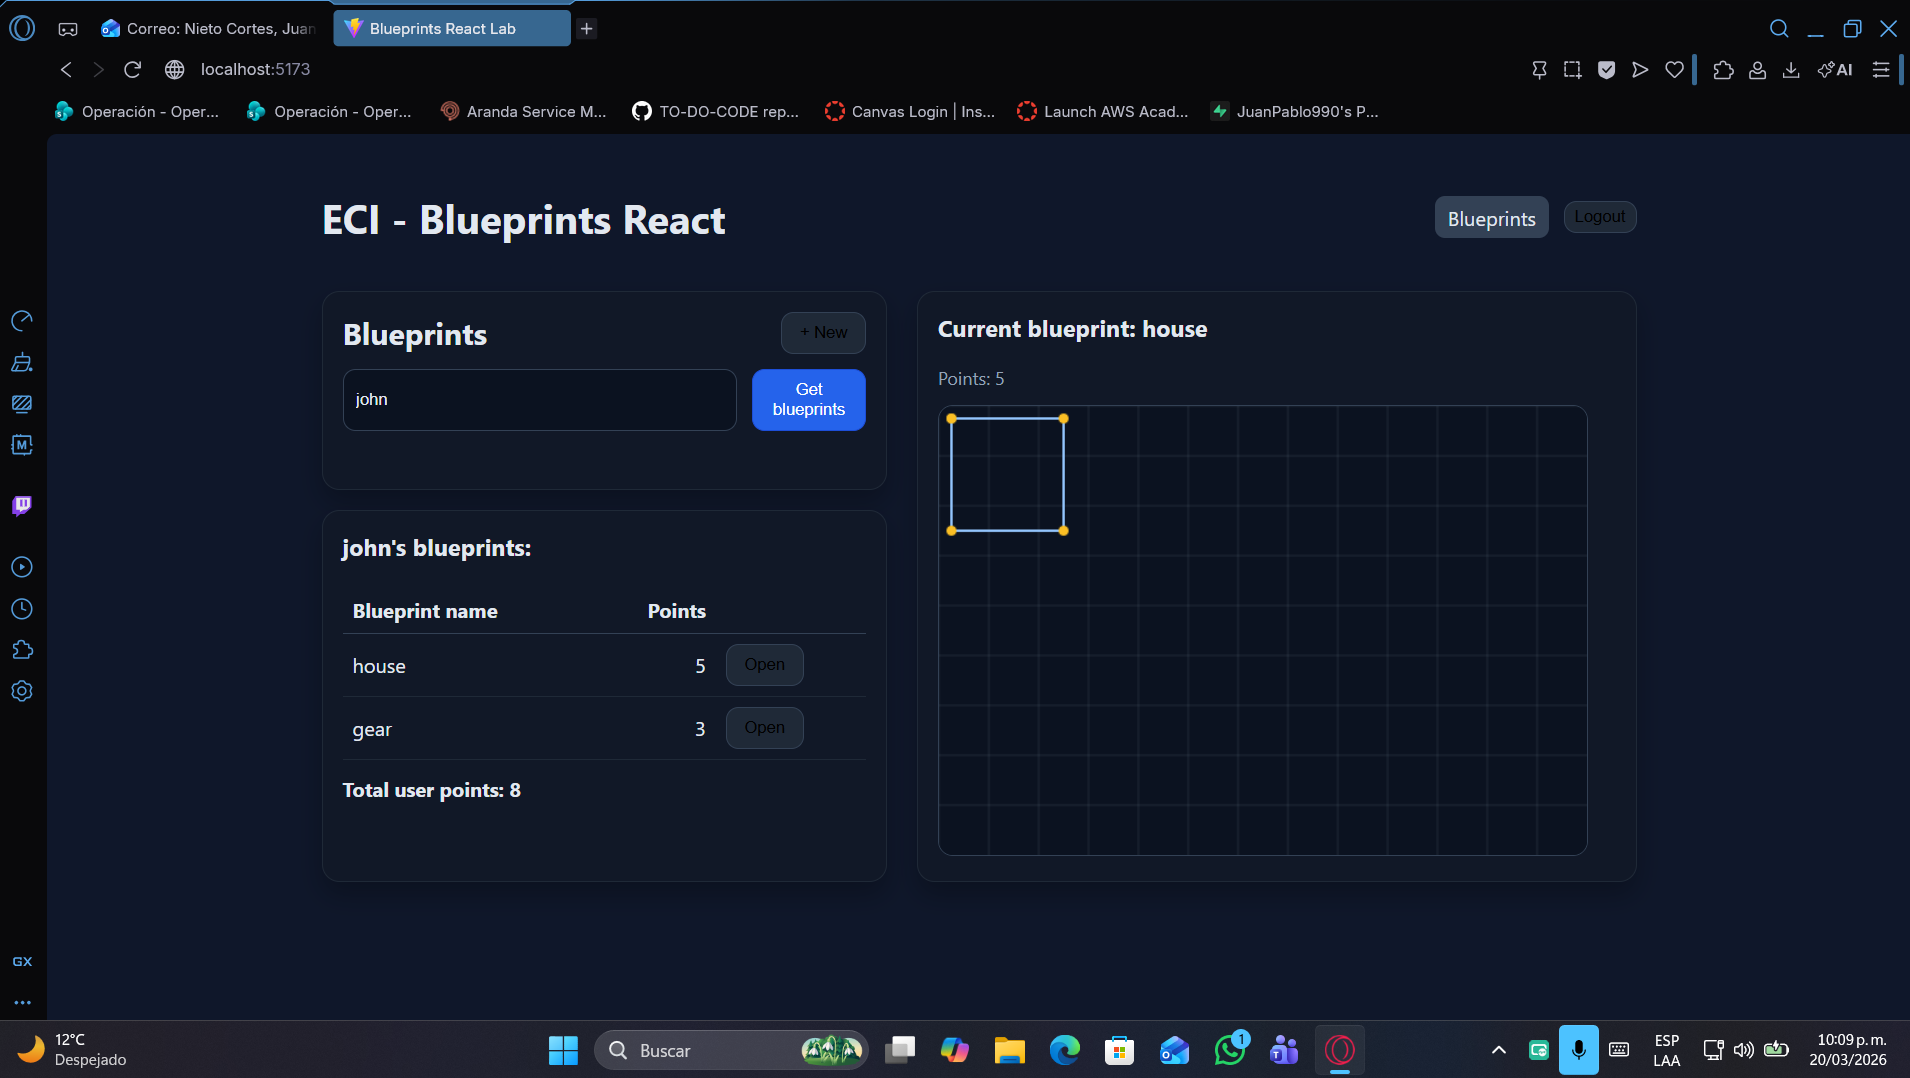
\includegraphics[width=0.9\textwidth]{canvas visualizacion.png}
    \caption{Figura 5: Visualización de la figura geométrica procesada en el Canvas}
\end{figure}

\newpage

\subsection{Persistencia: Creación de un Nuevo Plano}
Se validó la capacidad de enviar nuevos blueprints al sistema mediante el formulario integrado.
\begin{figure}[h]
    \centering
    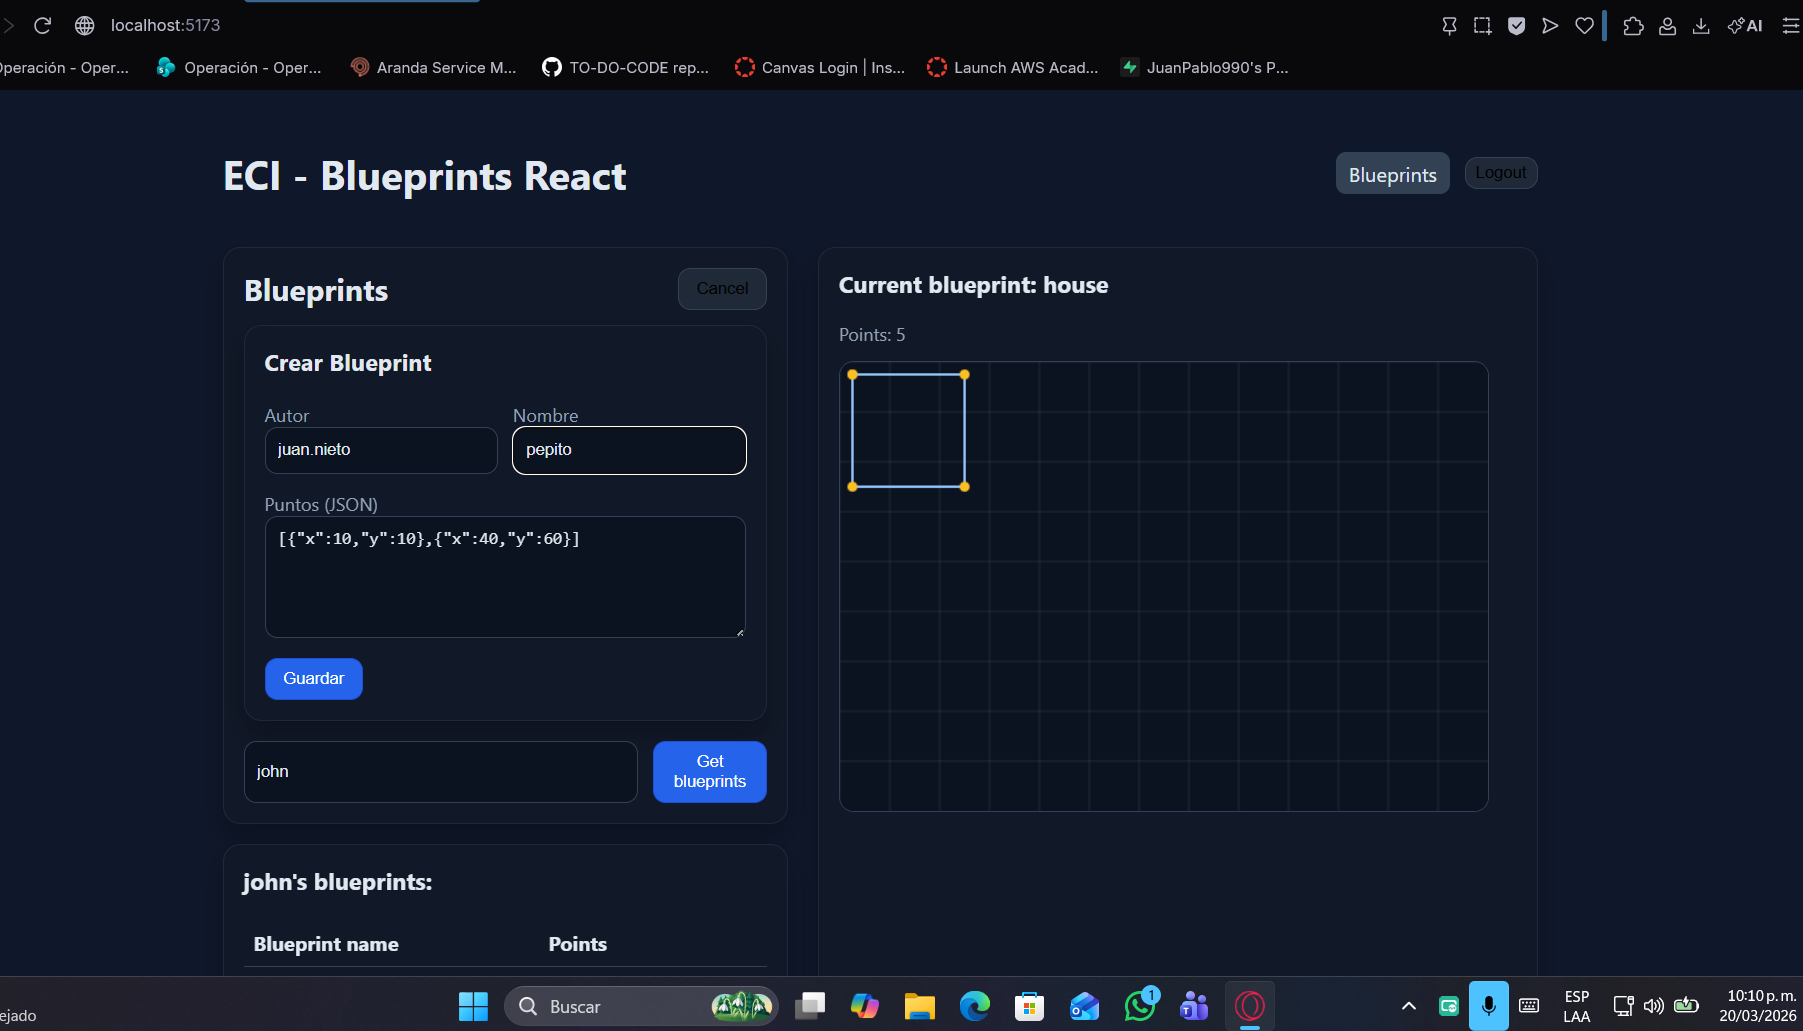
\includegraphics[width=0.9\textwidth]{nuevo plano.png}
    \caption{Figura 6: Solicitud POST para la creación exitosa de un blueprint}
\end{figure}

\newpage

\section{Conclusiones}
Basado en el desarrollo realizado para este laboratorio, se destacan las siguientes conclusiones técnicas:

\begin{itemize}
    \item Se logró implementar un cliente SPA seguro y funcional utilizando tecnologías de React y Redux Toolkit, cumpliendo con la arquitectura moderna de aplicaciones web.
    \item La integración de seguridad mediante JWT y el uso de interceptores RSA permitió establecer un mecanismo de autenticación robusto, escalable y acorde a las necesidades del proyecto.
    \item La arquitectura por capas implementada en el frontend, separando componentes, servicios y lógica de estado, facilitó significativamente la organización y mantenibilidad del código.
    \item El diseño de una capa de persistencia abstracta (Fachada de Servicios) permitió soportar almacenamiento Mock y producción sin acoplar los componentes visuales a la API.
    \item El uso de herramientas de calidad como Vitest, Docker y ESLint permitió desarrollar un producto final alineado con las mejores prácticas de la industria de software.
\end{itemize}

\newpage

\section{Resumen de la Entrega}
Este proyecto representa una solución integral para el Laboratorio 6, integrando todas las competencias adquiridas en el curso ARSW respecto al desarrollo de frontends modernos y seguros. La aplicación final no solo cumple con los requisitos funcionales mínimos, sino que ofrece una experiencia de usuario superior mediante el manejo riguroso de estados y errores.

\end{document}
